\section{Normal Estimation}
\label{section:normal-estimation}

Surface normals are an important property of geometric surfaces, and are fundamental for meshing algorithms and computer graphics, as for example, to calculate the shading and other visual effects\footnote{See "Estimating Surface Normals in a PointCloud" in \url{http://pointclouds.org/documentation/tutorials/normal_estimation.php}.}. As an example, the Stanford Bunny model\footnote{From \url{https://www.cc.gatech.edu/~turk/bunny/bunny.html}.} rendered with and without normals are show in \cref{figure:bunny-normals}. Normal estimation is quite trivial for surfaces, but for point clouds the process is quite not as easy. Usually there are two ways to estimate the normals: either by meshing the surface first, and then calculate the normals for the mesh, or using the point cloud itself to infer the normals. However, most meshing algorithms already require the normals to achieve a good result, so the latter option is more effective.

\begin{figure}[h]
    
    \centering
    \begin{subfigure}{0.4\textwidth}
        \centering
        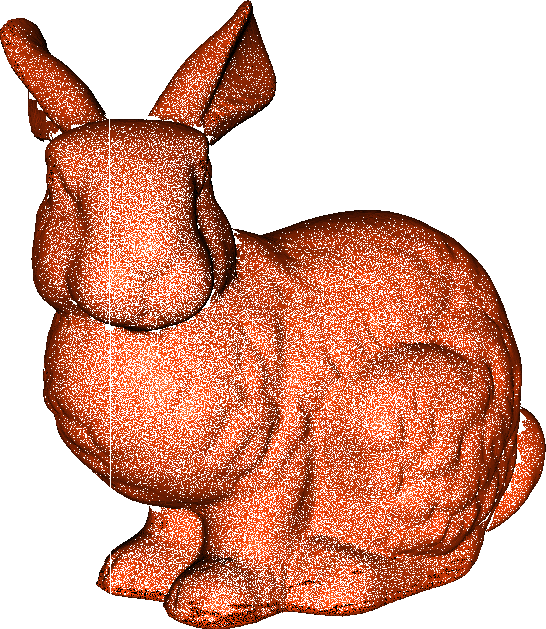
\includegraphics[height=6cm]{bunny-with-normals}     
    \end{subfigure}%
    \begin{subfigure}{0.4\textwidth}
        \centering
        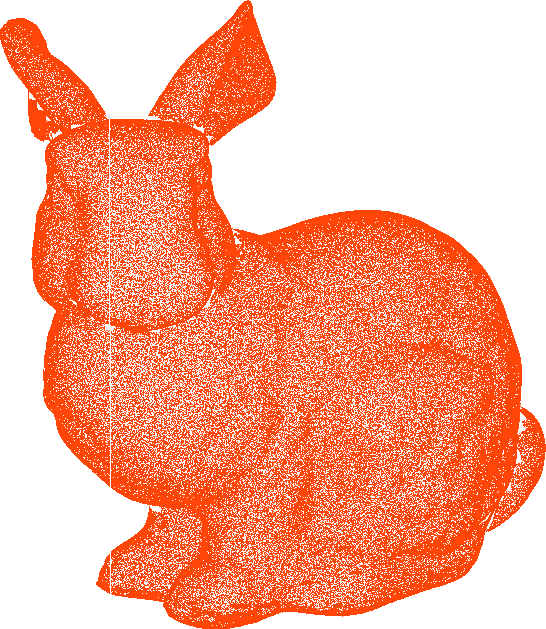
\includegraphics[height=6cm]{bunny-without-normals}     
    \end{subfigure}

    \caption{Stanford rabbit rendering with (left) and without (right) normals.}
    \label{figure:bunny-normals}

\end{figure}

The most common solution is, for each point, to find the $k$ closest point, defined as the $k$-neighborhood of a point, and calculate the normal of the best-fitting plane formed by this points. However, finding the $k$-neighborhood of all the points in a point cloud has a time complexity $O(N \log N)$, so it can become quite slow for point clouds with a large number of points. In this work, a new solution was used to find the closest points, exploiting the bidimensional structure of the point cloud. This solution has a linear time complexity $O(N)$, which makes it a valuable solution for large point clouds.

The solution were presented acknowledges that each point in the point cloud resulting from \cref{section:point-registration} has two indexes, one for the range index $i$ and one for the laser scan $j$. For each laser scan, each point $p_i$ has a neighborhood ${p_{i-k}, \ \dots, \ p_{i+k}}$, because each subsequent point has an increasing angle to the previous point. Between successive laser scans each point has an increasing angle (the pan angle) to the previous one. Therefore, for this algorithm, the neighborhood of each point is show in \cref{eqn:point-neighborhood}. The value of $k_1$ and $k_2$ have to be adjusted for a better result, because if the values are large, fine details are going to disappear and edges are going to be smeared, and on the other hand if the values are small, the surface will appear as too noisy.

\begin{equation}
\label{eqn:point-neighborhood}
    neighborhood(p_{i,j}, k_1, k_2) = \{p_{i-k_1, j-k_2}, \ \dots, \ p_{i+k_1, j+k_2}\}
\end{equation}

Then, for each point, the tangent plane that fits the neighborhood is calculated, which in turn is a least-square plane fitting problem. This is usually solved by an analysis of the eigenvalues and eigenvalues of the covariance matrix of the neighborhood points. This method is also known as the Principal Component Analysis.

To start with, for any neighborhood, the covariance matrix $\mathcal{C}$ is assembled as in \cref{eqn:covariance-matrix}, where $n$ is the number of points in the neighborhood and $\bar{p}$ is the centroid of these points. As before, an eigen-decomposition is performed in the covariance matrix to calculate the eigenvalues $\lambda_1, \lambda_2, \lambda_3$ and the corresponding eigenvectors $\texttt{v}_1, \texttt{v}_3, \texttt{v}_3$. Finally, the direction of the normal vector $n$ of the point is the eigen vector corresponding to the smallest eigenvalue, so $n = \pm \texttt{v}_3$.

Then, the orientation of the point has to be defined, because the result of the PCA is ambiguous, which may lead to inconsistent normals in the point cloud. In this case, the solution found was to orientate the normals towards the frame of the 3D scanner, which for each acquisition if the zero position.     Therefore, each normal has to satisfy the \cref{eqn:normal-orientation}.

\begin{equation}
\label{eqn:normal-orientation}
    n \cdot p < 0
\end{equation}

Further, there should be some filtering, specially for points at an edge, because the neighborhoods method described here is going to fail in this case. So, a proposed solution is to reject any point that exceeds a certain threshold distance to the center point. This has the advantage that the normal estimation can still work in the edges.